
%(BEGIN_QUESTION)
% Copyright 2013, Tony R. Kuphaldt, released under the Creative Commons Attribution License (v 1.0)
% This means you may do almost anything with this work of mine, so long as you give me proper credit

The following schematic diagram shows a Westinghouse model CO-11 overcurrent protective relay, complete with time-overcurrent (``CO''), instantaneous overcurrent (``IIT''), and seal-in (``ICS'') elements.  The relay as shown has been removed from service:

$$\includegraphics[width=15.5cm]{i02057x01.eps}$$

Suppose you were asked to test this relay to ensure it performs both the ``50'' and the ``51'' protective functions as designed.  When in service, this relay is connected to a current transformer having a ratio of 400:5 amps, and it is supposed to trip the breaker if the power line current exceeds 950 amps (for any length of time), or trip the breaker in 4.6 seconds if the power line current is at a value of 376 amps.  Explain in detail how you would bench-test this relay to ensure it is properly calibrated and functional for this application.

\vskip 20pt \vbox{\hrule \hbox{\strut \vrule{} {\bf Suggestions for Socratic discussion} \vrule} \hrule}

\begin{itemize}
\item{} Supposing you had no access to any precision protective relay calibration equipment, how could you build a simple circuit to generate the precise amounts of AC current needed to simulate overload conditions?
\end{itemize}

\underbar{file i02057}
%(END_QUESTION)





%(BEGIN_ANSWER)

To test the ``50'' (instantaneous overcurrent) function, apply 11.875 amps AC to terminals 3 and 8 (or terminals 8 and 9) with an ohmmeter connected to terminals 2 and 10 to check for the IIT contact's closure.  Of course, you would also need to re-test the relay at current values below 11.875 amps AC to verify that the relay does {\it not} pick up at any lower current value.
 
\vskip 10pt

To test the ``51'' (time overcurrent) function, apply 4.70 amps AC to terminals 8 and 9 with an ohmmeter connected to terminals 1 and 10 to check for the CO contact's closure after 4.6 seconds' worth of time.  
 
%(END_ANSWER)





%(BEGIN_NOTES)


%INDEX% Electric power systems: protective relays (time-overcurrent)
%INDEX% Protective relay: instantaneous overcurrent (50)
%INDEX% Protective relay: time-overcurrent (51)

%(END_NOTES)


